\tikzset{every picture/.style={line width=0.75pt}}    

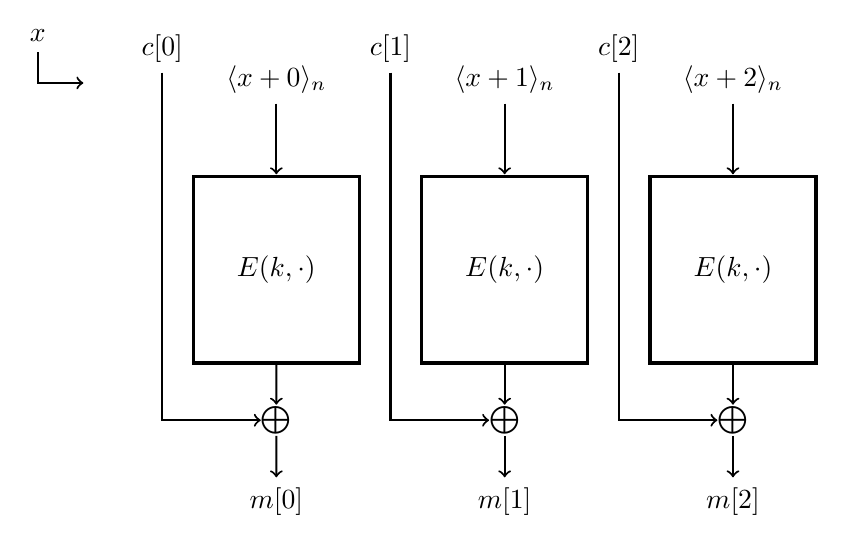
\begin{tikzpicture}[x=0.75pt,y=0.75pt,yscale=-1,xscale=1]

\draw  [line width=1.2]  (90,80) -- (170,80) -- (170,170) -- (90,170) -- cycle ;
\draw  [line width=1.2]  (200,80) -- (280,80) -- (280,170) -- (200,170) -- cycle ;
\draw  [line width=1.2]  (310,80) -- (390,80) -- (390,170) -- (310,170) -- cycle ;

\draw  [->]  (130,45) -- (130,79) ;
\draw  [->]  (240,45) -- (240,79) ;
\draw  [->]  (350,45) -- (350,79) ;
\draw  [->]  (130.03,170) -- (130,190) ;
\draw  [->]  (130.03,205) -- (130,225) ;
\draw  [->]  (240,170) -- (240,190) ;
\draw  [->]  (240,205) -- (240,225) ;
\draw  [->]  (350,170) -- (350,190) ;
\draw  [->]  (350,205) -- (350,225) ;
\draw  [->]  (75,30) -- (75,197.5) -- (122.5,197.5) ;
\draw  [->]  (185,30) -- (185,197.5) -- (232.5,197.5) ;
\draw  [->]  (295,30) -- (295,197.5) -- (342.5,197.5) ;
\draw  [<-]  (37,35) -- (15,35) -- (15,20) ;

\draw (130,125) node    {$E( k,\cdot )$};
\draw (75,26.6) node [anchor=south] [inner sep=0.75pt]    {$c[ 0]$};
\draw (130.03,228.4) node [anchor=north] [inner sep=0.75pt]    {$m[ 0]$};
\draw (240,125) node    {$E( k,\cdot )$};
\draw (185,26.6) node [anchor=south] [inner sep=0.75pt]    {$c[ 1]$};
\draw (240,228.4) node [anchor=north] [inner sep=0.75pt]    {$m[ 1]$};
\draw (350,125) node    {$E( k,\cdot )$};
\draw (295,26.6) node [anchor=south] [inner sep=0.75pt]    {$c[ 2]$};
\draw (350,228.4) node [anchor=north] [inner sep=0.75pt]    {$m[ 2]$};
\draw (130,197.5) node    {$\bigoplus $};
\draw (240,197.5) node    {$\bigoplus $};
\draw (350,197.5) node    {$\bigoplus $};
\draw (130,41.6) node [anchor=south] [inner sep=0.75pt]    {$\langle x+0\rangle _{n}$};
\draw (240,41.6) node [anchor=south] [inner sep=0.75pt]    {$\langle x+1\rangle _{n}$};
\draw (350,41.6) node [anchor=south] [inner sep=0.75pt]    {$\langle x+2\rangle _{n}$};
\draw (15,16.61) node [anchor=south] [inner sep=0.75pt]    {$x$};

\end{tikzpicture}